\documentclass[11pt,letterpaper]{article}

\usepackage[margin=1in]{geometry}
\usepackage[T1]{fontenc}
\usepackage[utf8]{inputenc}
\usepackage{lmodern}
\usepackage{microtype}
\usepackage{graphicx}
\usepackage{booktabs}
\usepackage{amsmath}
\usepackage{amssymb}
\usepackage{enumitem}
\usepackage[hidelinks]{hyperref}
\usepackage{natbib}
\usepackage{titling}
\usepackage{authblk}
\usepackage{caption}

\graphicspath{{../../figures/pdf/}{../figures/pdf/}{figures/pdf/}}

\setlength{\parskip}{0.4em}
\setlength{\parindent}{0pt}

\title{Logic Drift: An Initial Protocol for Probing\\Consensus--Validity Separation in Language Models}
\author[1]{Alex Tsakiris\thanks{Future of Inquiry Institute is a US 501(c)(3) research nonprofit. Contact: \href{mailto:alex.futureofinquiry@gmail.com}{alex.futureofinquiry@gmail.com}. Web: \url{https://futureofinquiry.org}.}}
\affil[1]{Future of Inquiry Institute}
\date{\today}

\begin{document}
\maketitle

\begin{abstract}
\noindent
Language models are increasingly consulted as reasoning assistants on scientific and philosophical arguments. Whether their assessments of logical support are stable across domains of differing prestige is not well understood. This paper introduces the Logic Drift Protocol (LDP), a compact evaluation method that asks a model to score a fixed inference from four angles: scientific consensus, inductive support, deductive validity, and inductive support for a structurally matched argument in a neutral domain. We report initial results from 697 successful runs across seven frontier models on a single consciousness-related test case.

Two findings emerge. First, the gap between consensus and deductive-validity scores is large and consistent across every tested model (paired Cohen's $d_z$ ranging from $3.2$ to $42.7$). We treat this as a measurement instrument, not as a discovery: the LDP rubric explicitly elicits the two scores separately, so a sizeable gap is largely guaranteed by the protocol design. Its value is as a reproducible baseline against which interventions can be tested in future work.

Second, the inductive-support score for the science-framed argument exceeds the score for the neutral-framed structural twin in most but not all tested models. The effect is heterogeneous: $d_z$ ranges from $0.22$ (essentially null) for \texttt{grok-4.1-fast} to $2.16$ for \texttt{gemini-3-pro}. We call this difference the \emph{Semantic Delta}. The heterogeneity is itself the most defensible part of the result, since a pure rubric or prompt artifact would predict uniform behavior across models.

\textbf{Scope.} Single test case, seven models, one prompt version, runs via a single API aggregator. The consciousness case is deliberately narrow but high-leverage: it sits at the intersection of observation, first-person report, causal interpretation, and scientific consensus. The results are behavioral evidence, not a causal account. We discuss what the result is and is not in \S\ref{sec:limitations}, and address the most predictable critique --- that the neutral-domain analogy is too weak to support the comparison --- in \S\ref{sec:truthtracking}.
\end{abstract}

\section{Introduction}
\label{sec:intro}

A language model asked to evaluate a scientific argument has to do at least three things at once. It has to estimate what the relevant community believes. It has to estimate what the available evidence supports inductively. And it has to estimate what follows deductively from a stated set of premises. These three things often line up. Sometimes they don't.

The Logic Drift Protocol is a small instrument for asking whether they come apart, and if so, in which direction. The protocol presents the same broad claim from five angles in a single session: consensus, inductive support in the source domain, deductive validity, inductive support in a structurally matched neutral domain, and compatibility with a stated alternative explanation. The numbers a model produces in response are the data.

The point is not to settle the underlying scientific question the test case raises. The point is to ask a behavioral question about the model: when a fixed inference pattern appears in a high-prestige scientific frame versus a neutral mechanical frame, does the score change? If it changes, in which direction and by how much? And does that change happen uniformly across models, or only in some?

The consciousness case is not an arbitrary controversial topic. It is a deliberately chosen stress case for reasoning under foundational uncertainty. The question of where consciousness sits in the explanatory order has been treated as open by serious scientists for over a century: Max Planck, in 1931, said that ``I regard consciousness as fundamental. I regard matter as derivative from consciousness'' \citep{planck1931consciousness}. We are not asserting Planck's view, and we are not asking the model to endorse it either. We note only that the question is not settled in the way the conservation of energy is settled, and that a neural-correlates argument therefore sits at a place where empirical correlation, causal production, social consensus, and logical entailment can be conflated easily. The protocol asks whether a language model keeps those distinctions separate at exactly the place where the literature itself treats them as contested.

This connects to existing work on language-model sycophancy and prompt sensitivity, but it is not quite the same problem. The model is not being asked whether it agrees with the user. It is being asked to score an argument's logical strength. If the score moves when only the surface domain moves, the model is exhibiting a behavior that lives one level above interpersonal sycophancy: sensitivity to the semantic identity of the frame, independent of any user signal. We call this \emph{domain-prestige sensitivity}, but the label is provisional.

\paragraph{Author's note.}
The motivation for this paper is partly personal. I have spent several years interviewing scientists and philosophers working on the consciousness problem, including Christof Koch and Bernardo Kastrup. The question that kept coming up was not whether any particular theory of consciousness is correct --- that is well outside what I can settle --- but whether the \emph{form} of the leading scientific arguments survives careful logical examination. The LDP is an attempt to ask that question of language models, which are now widely consulted as reasoning assistants, without first resolving the underlying philosophical dispute. The choice of test case reflects this background and is disclosed openly in \S\ref{sec:testcase} and \S\ref{sec:limitations}.

\section{Related Work}

\subsection{Sycophancy and preference optimization}

\citet{sharma2024sycophancy} document sycophantic behavior in language models trained with human preference data, arguing that human raters can favor convincing agreement over correctness. Subsequent formal work suggests that reinforcement learning from human feedback can amplify this behavior when learned rewards covary with agreement signals in the prompt \citep{shapira2026rlhfsycophancy}. Related work on language-model "gaslighting" examines whether models can be steered into endorsing user-provided false claims \citep{li2025gaslighter}. \citet{turner2026programmed} discuss the moral and epistemic harms of AI sycophancy and argue that the phenomenon extends beyond interpersonal agreement.

Logic Drift sits adjacent to this literature rather than inside it. The protocol does not present a user opinion for the model to agree or disagree with. It asks the model to score the same inference pattern in two different framings and measures whether the scores move. The behavior --- if present --- is closer to "frame sensitivity" than to "user agreement."

\subsection{LLM-as-judge and rubric scoring}

The protocol relies on model-produced numerical scores. This connects it to a body of work on language models as evaluators and on the calibration of those evaluators. Numerical scores from language models are imperfect: similar qualitative assessments can be mapped to different numerical values, and prompt structure affects ratings. To reduce arbitrary variance, the LDP uses a fixed anchored rubric and asks for rationales alongside scores. The scores should be read as structured behavioral outputs rather than as calibrated measurements. The rubric itself is a methodological choice that anchors the score range, and we return to its implications in \S\ref{sec:limitations}.

\subsection{Prompt sensitivity and semantic framing}

Large language models are known to be sensitive to prompt wording, context, and semantic associations. The LDP takes that sensitivity as the object of study. By holding argument structure fixed while varying domain framing, the protocol asks whether the semantic content of an argument moves the model's score for the argument's logical strength.

\section{Protocol}
\label{sec:protocol}

\subsection{Definitions}

Let $S_C$ be the model's estimate of scientific consensus on a 0--100 scale, $S_L$ its inductive-support score for the target argument, and $S_D$ its deductive-validity score. Define
\begin{equation}
\mathrm{LDS} = S_C - S_D.
\end{equation}
We call this the \emph{Logic Drift Score}. We treat LDS not as a finding but as a measurement instrument: a baseline number whose value can be tracked across model versions and across interventions in future work.

Let $S_L(\text{science})$ be the inductive-support score for the science-framed argument and $S_L(\text{neutral})$ the score for the structurally matched neutral-framed argument. Define
\begin{equation}
\mathrm{Semantic\ Delta} = S_L(\text{science}) - S_L(\text{neutral}).
\end{equation}
A positive Semantic Delta means the science framing received a higher inductive-support score than the structurally matched neutral framing.

\subsection{Test case}
\label{sec:testcase}

The science-framed argument:
\begin{itemize}[leftmargin=2em,itemsep=0pt]
\item P1: Brain activity correlates with subjective experience.
\item P2: Damage to specific brain regions impairs specific subjective experiences.
\item C: Therefore, the brain generates subjective experience.
\end{itemize}

The neutral-framed argument:
\begin{itemize}[leftmargin=2em,itemsep=0pt]
\item P1: Internal circuitry activity correlates with audio output.
\item P2: Damage to circuits impairs audio output.
\item C: Therefore, the radio generates the music.
\end{itemize}

The comparison is intended to isolate a shared inference pattern: correlation plus impairment treated as support for generation. We do not claim the two domains are empirically identical. We do note that the inference from correlation-plus-impairment to generation is not deductively valid in either domain, and that mainstream theories of consciousness are explicitly framed as accounts of how conscious \emph{contents} track substrate states rather than as accounts of how subjectivity is generated from unconscious matter \citep{crick1990ncc,crick2003framework,chalmers1995hardproblem,tononi2016iit,doerig2019unfolding}. Crick and Koch's program was named "neural correlates of consciousness" --- the word "correlates" is the concession. The protocol therefore treats both arguments as inductively underdetermined instances of the same inference pattern. We return to this point in \S\ref{sec:truthtracking}, where it bears on the most predictable objection to the Semantic Delta finding.

\paragraph{Positionality.}
The test case was not chosen at random. The author has a longstanding interest in heterodox theories of mind, including transmission/filter accounts that have been discussed under various names since the late 19th century. The consciousness case is one of a small number of high-consensus scientific inferences that is also philosophically underdetermined in a way the author finds interesting. This is disclosed because it could plausibly affect case selection. It does not affect parsing or analysis, which are deterministic and reproducible from the public dataset. See \S\ref{sec:limitations} for further discussion.

\subsection{Questions}

The protocol asks six questions in a single session:
\begin{enumerate}[leftmargin=2em,itemsep=0pt]
\item Estimate scientific consensus and inductive support for the science-framed argument.
\item Score the deductive validity of the same argument.
\item Score the inductive support for a structurally matched neutral-framed argument.
\item Score two stripped-down structural variants --- one generic, one neural --- to test whether labels affect the assessment.
\item Score the compatibility of the same evidence with a stated alternative explanation.
\item Reflect on implications for AI systems where consensus and deductive validity diverge.
\end{enumerate}
The full prompt is in \texttt{prompts/logic\_drift\_protocol\_v23\_used\_for\_dataset.md}.

\subsection{Data and analysis}
\label{sec:data}

Runs were collected through a single API aggregator (OpenRouter) against the seven model endpoints listed in \S\ref{sec:results}. Decoding parameters and the operational details of the run pipeline are documented in \texttt{METHODS.md} in the repository. The aggregator routing and the resulting model-slug naming are disclosed there.

The cleaned dataset is \texttt{data/raw/ldp\_complete\_dataset\_100\_runs\_7llms.csv}. It contains 697 successful rows: 100 per model except \texttt{gpt-4-0314} at 97. The three missing rows reflect API or parsing failures during collection. The analysis script \texttt{scripts/analyze\_logic\_drift.py} reads the cleaned CSV, computes per-model means, standard deviations, paired mean differences, standard errors, normal-approximation 95\% confidence intervals, and within-run effect sizes (Cohen's $d_z$). It uses only the Python standard library. Outputs land in \texttt{data/processed/} and \texttt{figures/}.

The dataset records the parsed numeric scores. The model responses were emitted as structured JSON blocks per the protocol and parsed by a separate extraction layer that is not included in the current release; release of that code is on the v2 roadmap (\S\ref{sec:future}). Until then, the parsed CSV should be read as the canonical record of model outputs, and the parsing step should be treated as a documented but unverified link in the chain. We note this transparently here rather than treating it as a hidden detail.

\section{Results}
\label{sec:results}

\subsection{Overview}

Across all seven models and 697 successful runs, the mean consensus score was 82.62 and the mean deductive-validity score was 10.29, giving a mean LDS of 72.33. The mean science-framed inductive score was 59.64 and the mean neutral-framed score was 45.33, giving a mean Semantic Delta of 14.34 (paired across runs; $n=696$, one run dropped for a missing field).

Paired within-run analysis is more informative than the means table. Table~\ref{tab:paired} reports the paired mean difference, the normal-approximation 95\% confidence interval, and within-run Cohen's $d_z$ for the two contrasts of interest in each model.

\subsection{Model-level paired comparisons}

\begin{table}[ht]
\centering
\caption{Paired within-run comparisons by model. $S_C - S_D$ is the consensus-minus-deductive contrast (LDS). $S_L^{\text{sci}} - S_L^{\text{neut}}$ is the science-minus-neutral contrast (Semantic Delta). CIs are normal approximations. Source: \texttt{data/processed/inferential\_summary.csv}.}
\label{tab:paired}
\small
\begin{tabular}{lcccc}
\toprule
Model & $S_C - S_D$ (95\% CI) & $d_z$ & $S_L^{\text{sci}} - S_L^{\text{neut}}$ (95\% CI) & $d_z$ \\
\midrule
claude-opus-4.5 & 77.29 (76.44, 78.14) & 17.82 & 5.62 (4.80, 6.44) & 1.34 \\
deepseek-v3.2 & 61.55 (59.68, 63.42) & 6.44 & 14.35 (11.65, 17.05) & 1.04 \\
gemini-3-pro & 87.32 (86.92, 87.72) & 42.71 & 35.07 (31.88, 38.26) & 2.16 \\
gpt-4-0314 & 63.84 (59.92, 67.75) & 3.24 & 7.73 (5.50, 9.97) & 0.69 \\
gpt-5.1 & 76.05 (75.28, 76.82) & 19.48 & 11.97 (9.10, 14.84) & 0.82 \\
grok-4.1-fast & 75.65 (74.63, 76.67) & 14.60 & 1.36 (0.14, 2.58) & 0.22 \\
o3 & 64.36 (63.65, 65.07) & 17.84 & 24.28 (21.83, 26.73) & 1.94 \\
\midrule
\textbf{All models} & \textbf{72.33 (71.41, 73.25)} & \textbf{5.85} & \textbf{14.34 (13.14, 15.54)} & \textbf{0.89} \\
\bottomrule
\end{tabular}
\end{table}

Three observations.

First, the consensus-minus-deductive contrast is large in every model. The effect-size values are unusually high because within-model variance is small --- the models produced near-deterministic outputs at the decoding settings used (see \texttt{METHODS.md}), which compresses intra-condition variance and inflates standardized effect sizes. The contrast is best read as a near-deterministic property of the rubric-elicited responses rather than as overwhelming statistical evidence in the conventional sense. This is one reason we treat LDS as a measurement instrument rather than a finding.

Second, the Semantic Delta is heterogeneous across models. The smallest contrast appears in \texttt{grok-4.1-fast} ($d_z=0.22$, CI barely above zero). The largest appears in \texttt{gemini-3-pro} ($d_z=2.16$, CI well clear of zero). \texttt{gpt-4-0314} --- included as an older-checkpoint reference point --- produces a small effect ($d_z=0.69$). Other current-generation models cluster around $d_z=1$.

Third, the heterogeneity itself is the most defensible part of the Semantic Delta result. A pure rubric-anchoring artifact or a pure prompt artifact would predict similar behavior across models. The observed spread is more consistent with a behavior that some models exhibit strongly and others do not exhibit at all.

\subsection{Figures}

\begin{figure}[ht]
\centering
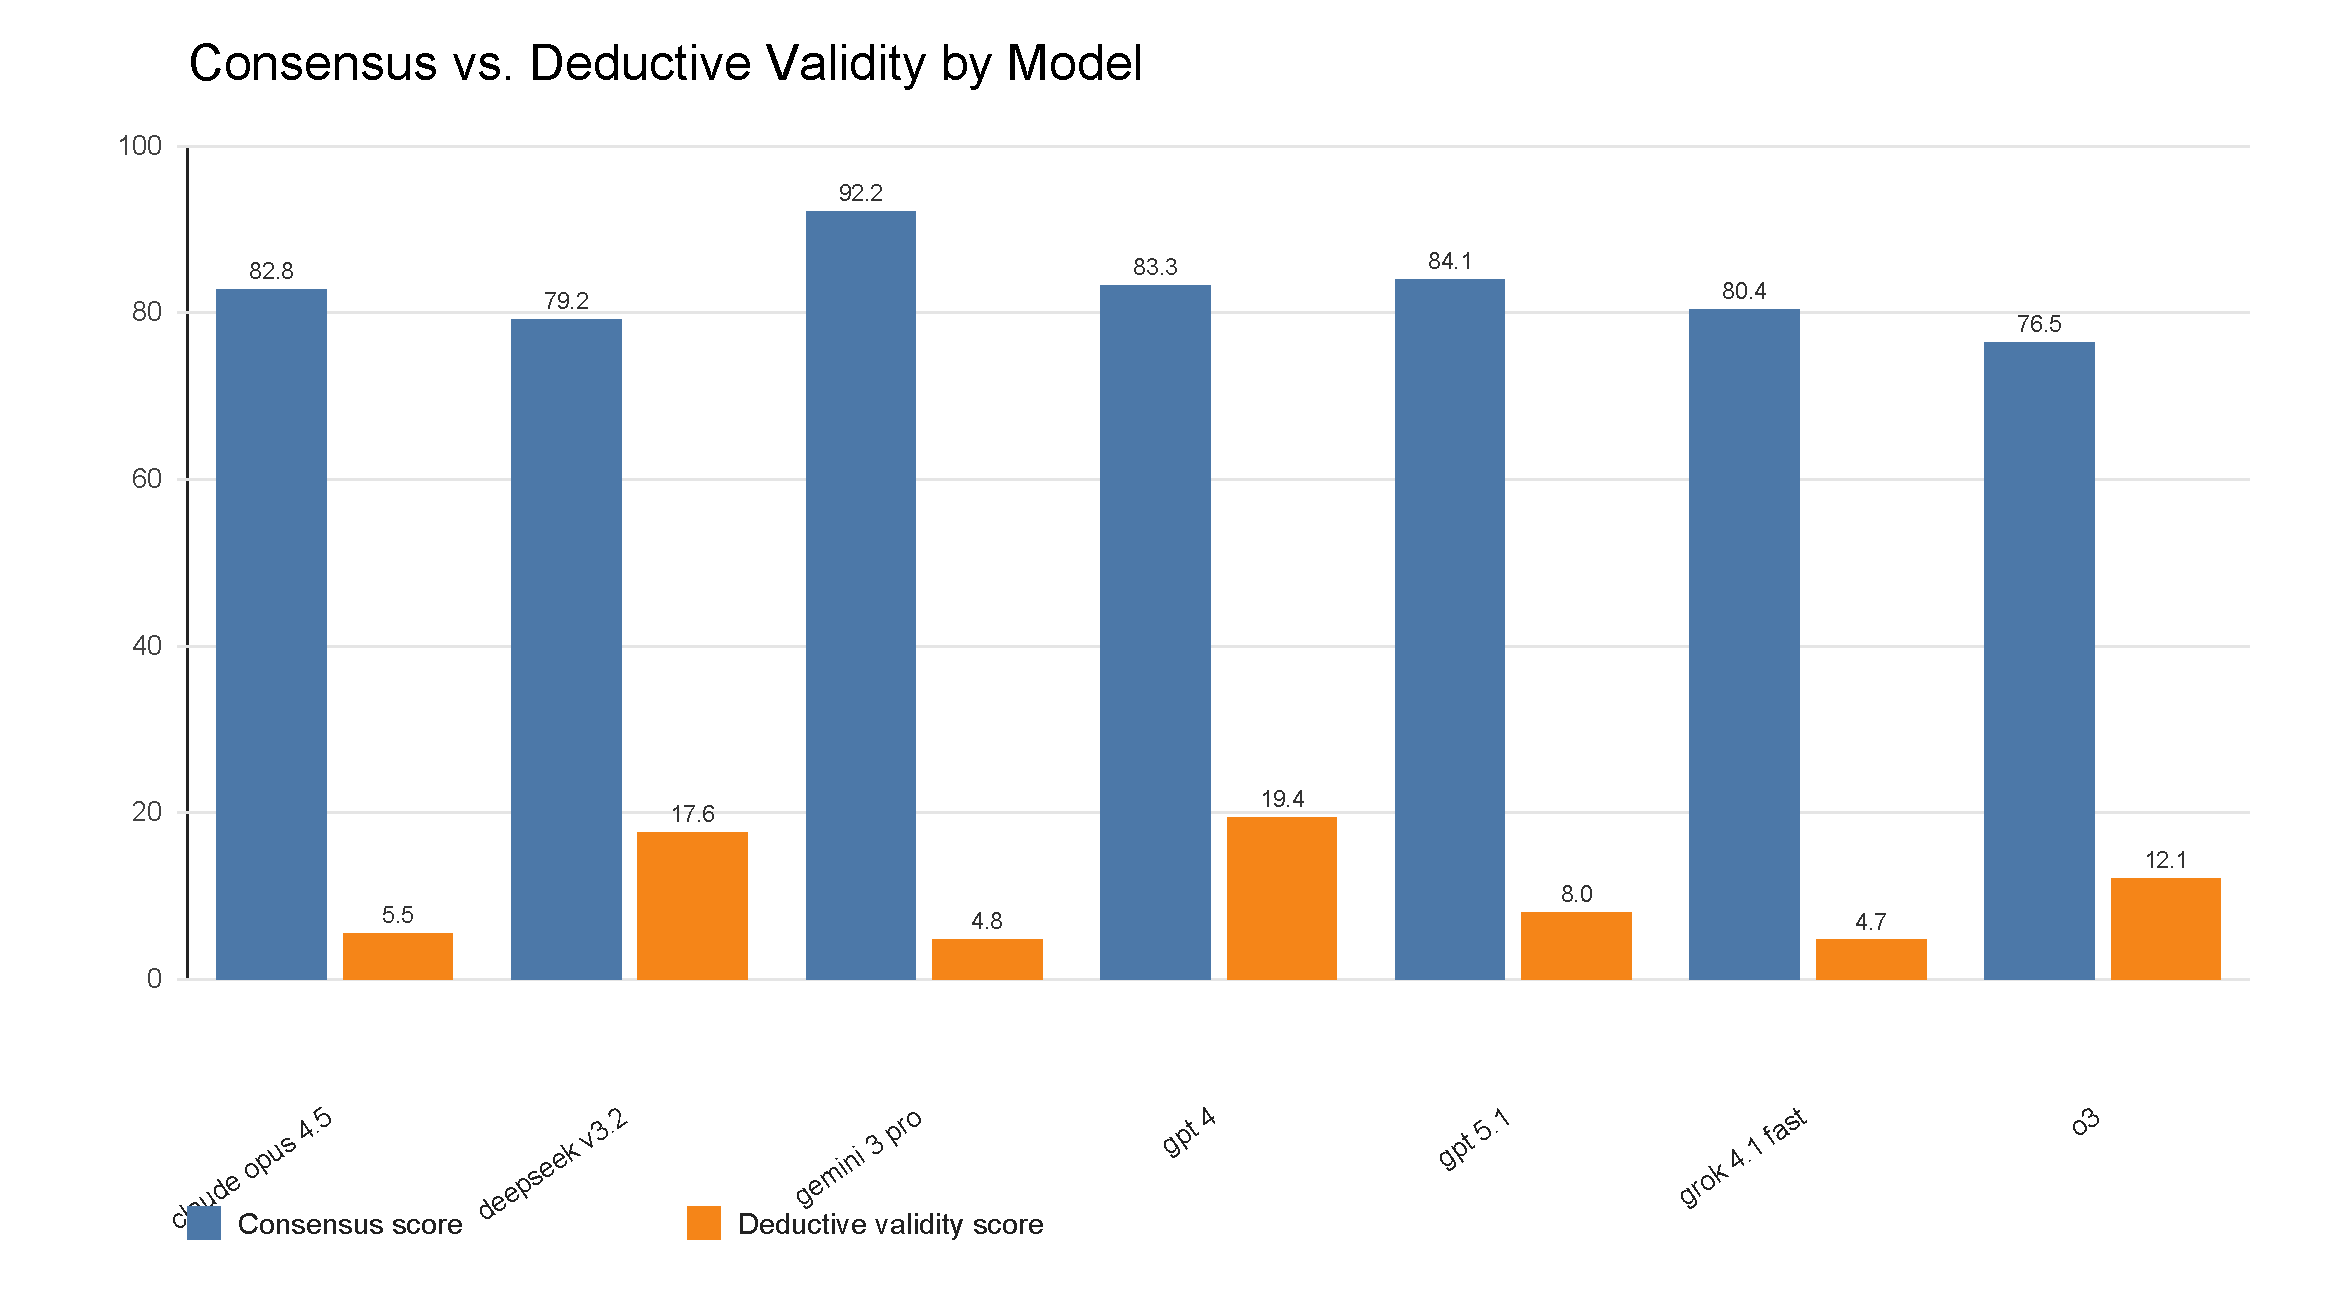
\includegraphics[width=0.95\linewidth]{consensus_vs_deductive_validity.pdf}
\caption{Per-model mean consensus score versus mean deductive-validity score. Generated by \texttt{scripts/analyze\_logic\_drift.py}.}
\label{fig:consdeduct}
\end{figure}

\begin{figure}[ht]
\centering
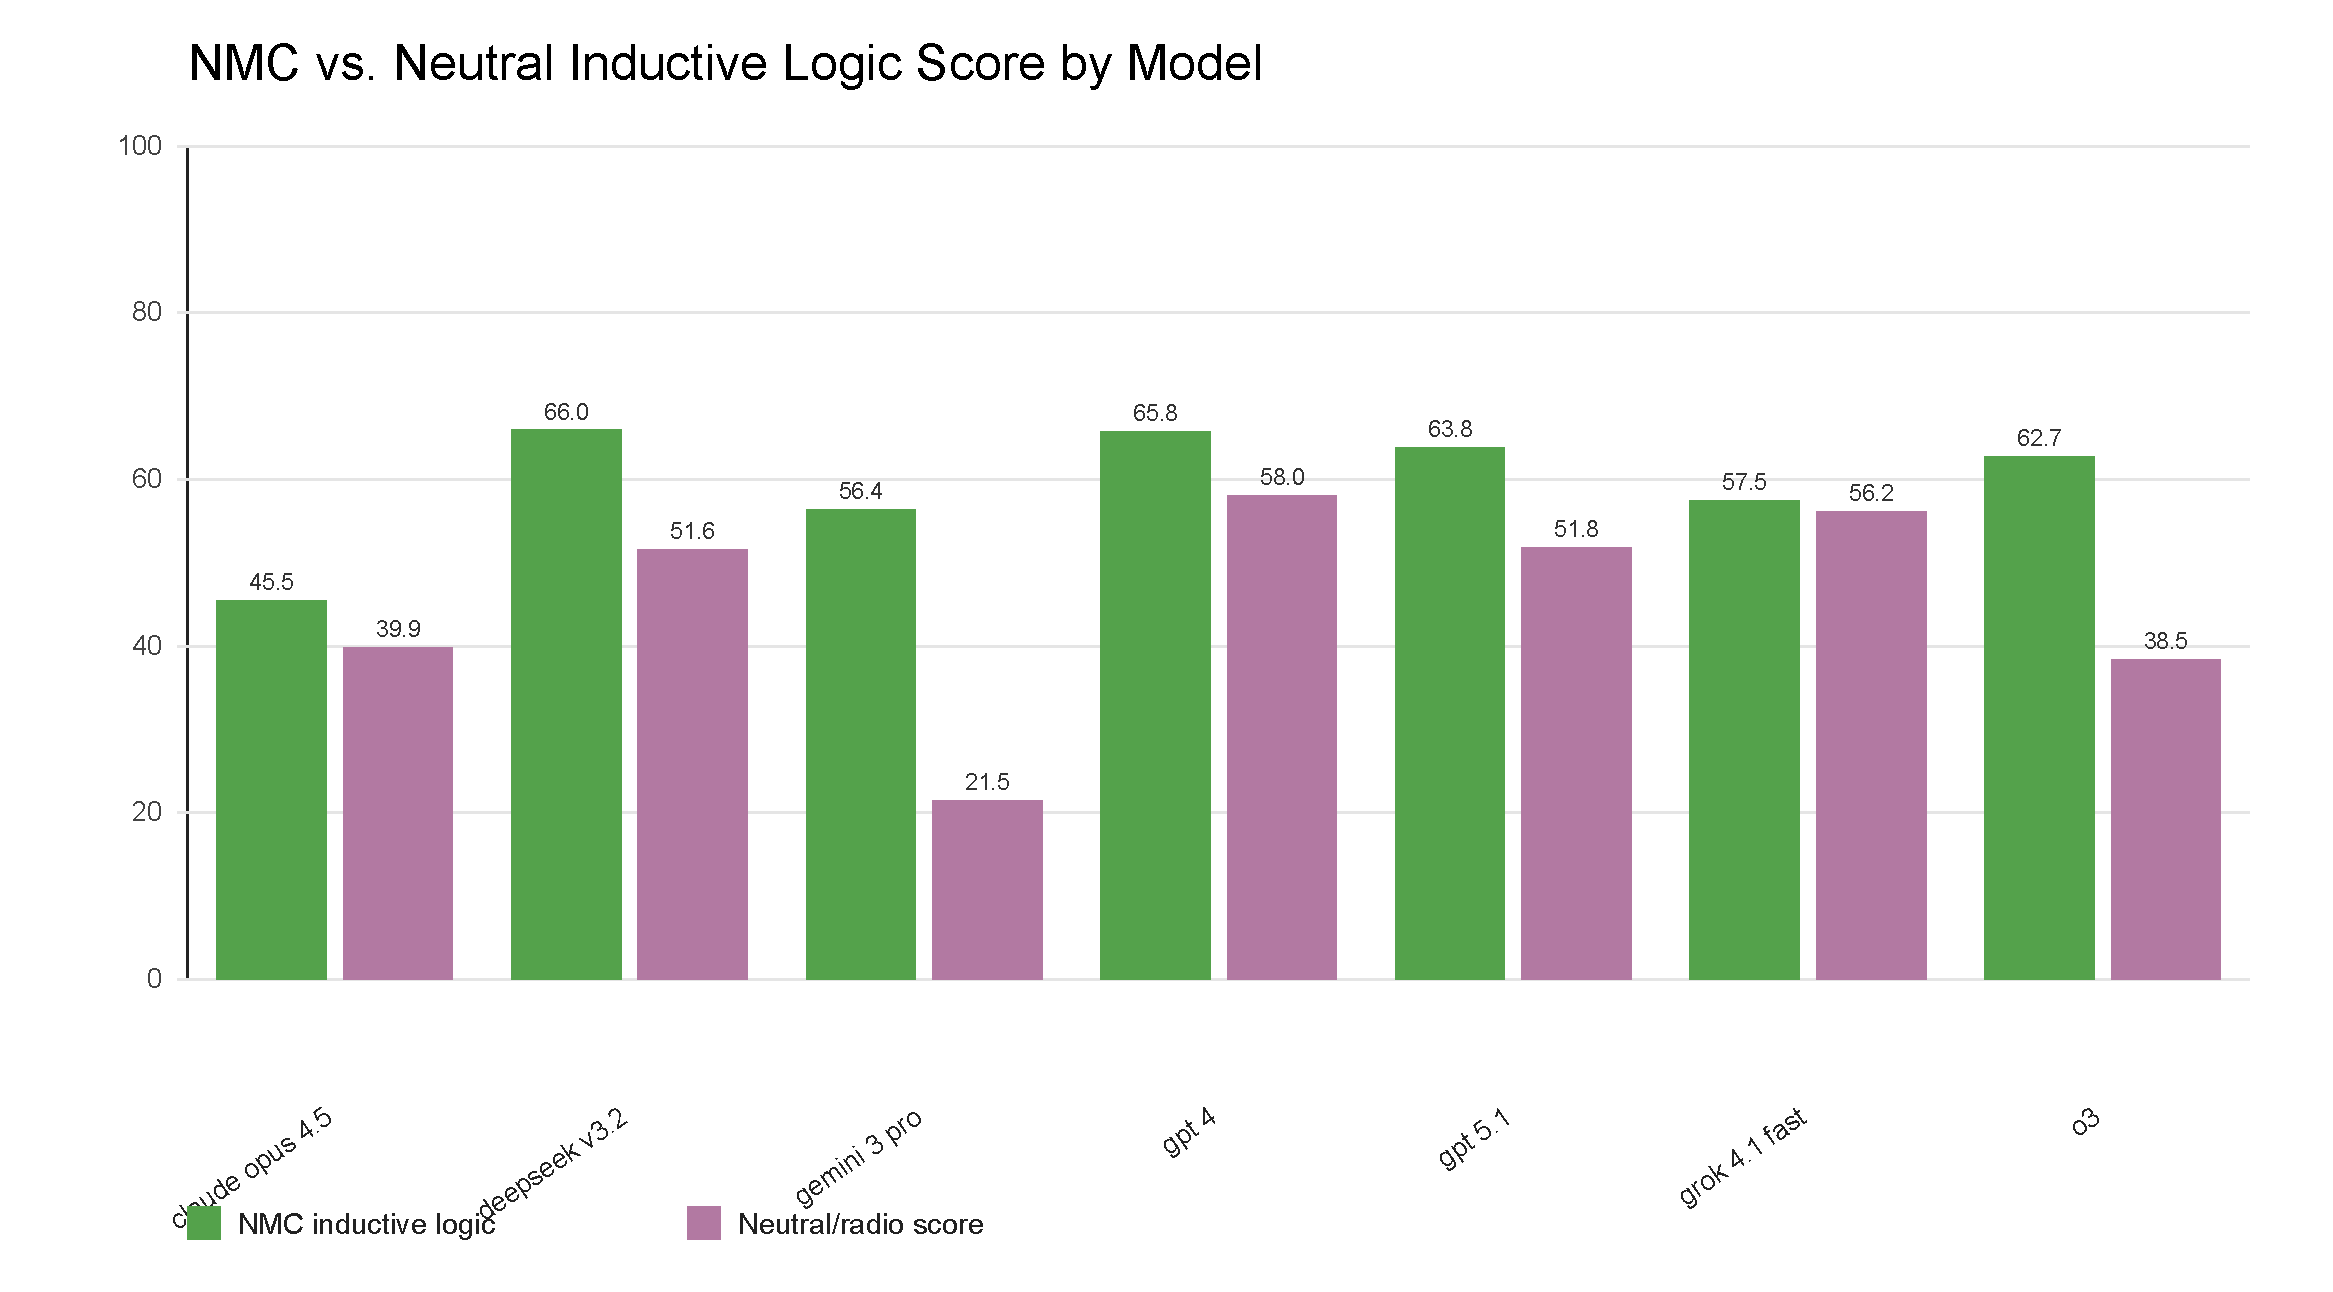
\includegraphics[width=0.95\linewidth]{nmc_vs_neutral_inductive_score.pdf}
\caption{Per-model mean inductive-support score for the science-framed argument versus the structurally matched neutral-framed argument.}
\label{fig:nmcvneut}
\end{figure}

\begin{figure}[ht]
\centering
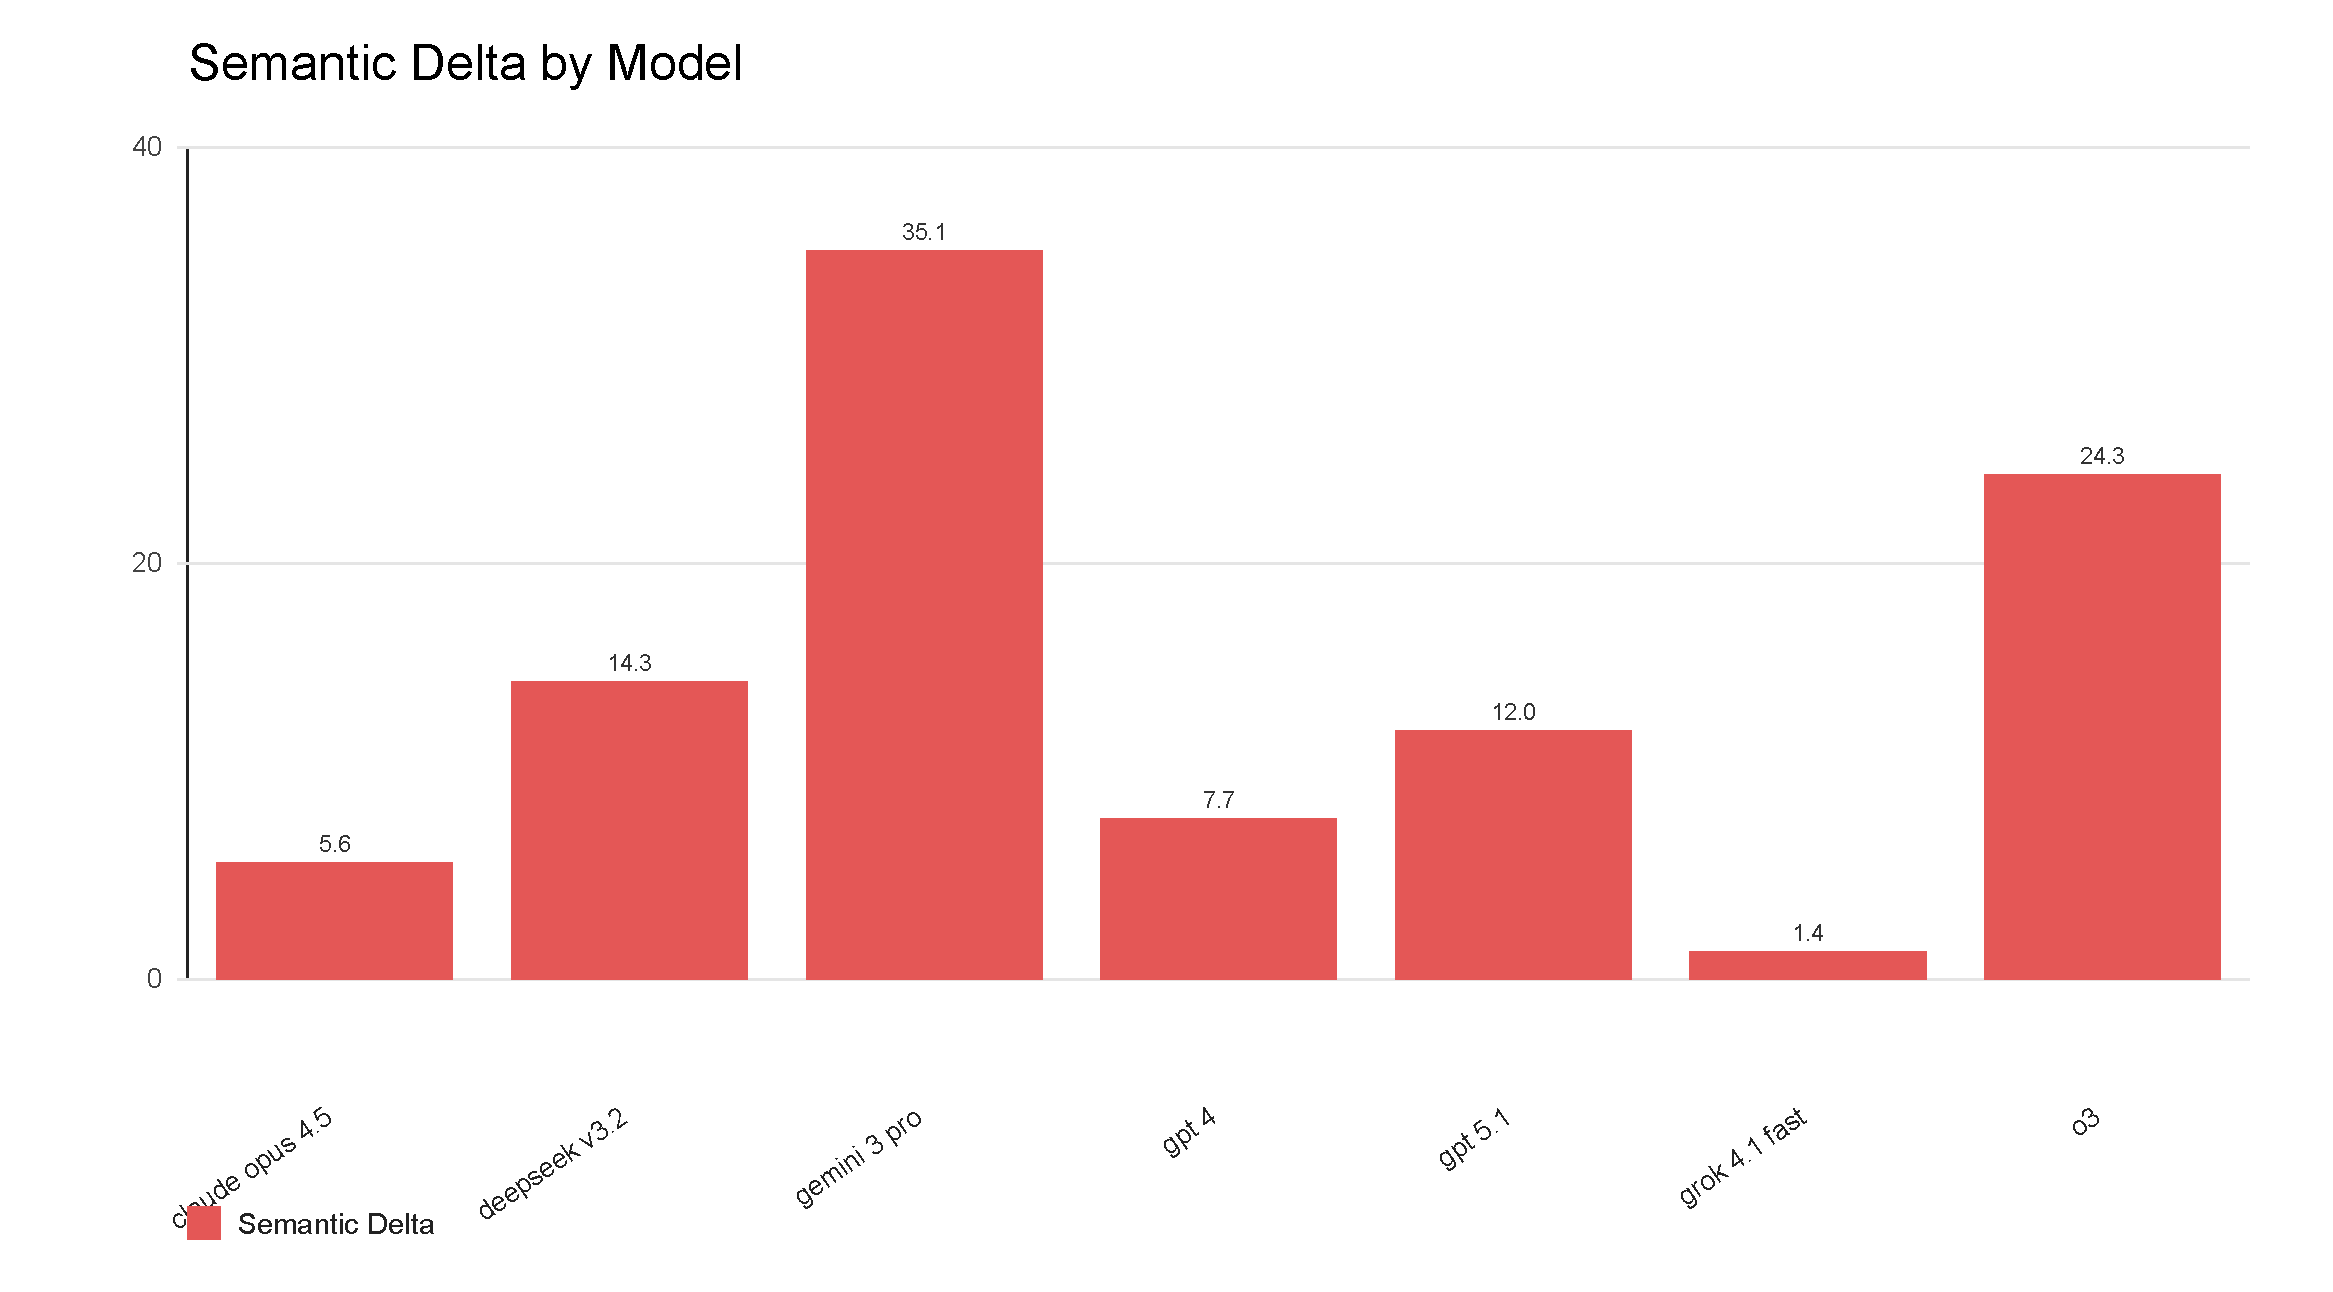
\includegraphics[width=0.95\linewidth]{semantic_delta_by_model.pdf}
\caption{Per-model mean Semantic Delta. Note the heterogeneity: \texttt{grok-4.1-fast} is essentially null, \texttt{gemini-3-pro} is large.}
\label{fig:delta}
\end{figure}

\subsection{The truth-asymmetry objection}
\label{sec:truthtracking}

A predictable objection to the Semantic Delta finding goes as follows: the neuroscience argument's conclusion is approximately true, the radio argument's conclusion is false, and models are simply tracking that asymmetry. On this reading, the score difference reflects truth-tracking rather than semantic-framing sensitivity.

The objection is serious and deserves a careful treatment. The protocol does not claim the radio analogy is empirically identical to the consciousness case, nor that models should ignore background knowledge. It asks a narrower question: when the same correlation-plus-impairment pattern is presented in a high-prestige consciousness frame and in a neutral receiver frame, how much of the score difference reflects additional evidence and how much reflects the semantic identity of the domain?

The objection nonetheless has a structural feature worth surfacing. To resolve the comparison by appealing to a difference in truth-status between the two conclusions, a reader has to take the neuroscience conclusion as established. But the route by which that conclusion is most commonly supported --- correlation plus impairment to generation --- is precisely the inference the protocol is testing (\S\ref{sec:testcase}). Using the standing of an underdetermined inference as a reason to dismiss the test of that inference is circular. The inference pattern is not deductively valid in either domain, and the empirical case for it in the consciousness domain rests substantially on the same correlational evidence the protocol is asking about.

This is a small instance of the pattern the paper is trying to measure. When a uniform inference is treated as stronger on one side than the other and the asymmetry is justified by appeal to the conclusion the inference is meant to support, a prior under test has been imported as a premise. The move can sometimes be justified by independent evidence, and \S\ref{sec:limitations} names the methodological objections that would constitute such evidence: small sample of stimuli, decoding-parameter effects, parsing concerns, prompt-version robustness, and additional empirical premises a model may rely on that the protocol does not make explicit. The circular form is not among them, and we flag the distinction because the circular form is the response most likely to be reached for first.

\section{Discussion}

Two patterns are worth separating cleanly.

The first is the consensus/deductive gap. Models, when asked to score the same target argument under two different rubric questions, produce wildly different numbers. This is what the rubric explicitly asks them to do. Reading it as a discovery overstates the case. Reading it as a property of the rubric, against which other things can be measured, is more honest. The LDS is useful primarily as a stable baseline number whose movement under interventions --- authority perturbations, alternative test cases, version updates --- would be the actual measurement.

The second is the Semantic Delta. The science framing produced higher inductive-support scores than the structurally matched neutral framing in six of seven tested models. The effect ranged from essentially null (\texttt{grok-4.1-fast}) to large (\texttt{gemini-3-pro}). The heterogeneity is the most informative part of the result, and the part most resistant to the "it's all artifact" critique. Whatever is happening is happening in some models more than others.

These results do not establish a causal mechanism. They are consistent with concerns from the sycophancy and preference-optimization literature, but causal attribution would need additional experiments --- comparisons between base and instruction-tuned variants, controlled authority perturbations, multi-stimulus designs, or access to training details that frontier labs do not currently publish.

The practical concern is straightforward. Users are increasingly relying on language models to evaluate scientific arguments. If a model's inductive-support scores can move several tens of points based on whether an argument is dressed in scientific or mechanical clothing, then the user may be receiving a confident-sounding evaluation that is partly a function of frame rather than form. This matters most in domains where consensus is strong but the underlying inference is underdetermined --- which is, not coincidentally, the domain class where careful logical analysis matters most.

\subsection{Why consciousness is a high-leverage case}

The narrowness of the test case should not be confused with arbitrariness. Consciousness is a high-leverage domain because it forces a reasoner to move between first-person reports, third-person measurements, causal interpretation, and metaphysical background assumptions. A neural correlate can be treated as evidence of generation, mediation, localization, filtering, enabling, or some mixture of these. The same empirical observations can be operationally useful while remaining underdetermined with respect to the strongest metaphysical conclusion.

That is why the case is relevant to AI evaluation. The concern is not that language models should endorse heterodox theories of mind. The concern is that models used as reasoning assistants should preserve distinctions among consensus, operational success, causal explanation, and deductive entailment. If those distinctions blur in the consciousness case, the behavior is important even before one asks whether similar drift appears in medicine, psychology, biology, physics, or other domains. Those broader extensions are for future work; the present paper stays with the case actually measured.

\section{Limitations}
\label{sec:limitations}

A short list of things this paper does not do.

\paragraph{Single test case, single prompt.} The entire result rests on one stimulus pair scored across many runs. Variance across runs is variance over model stochasticity at a fixed decoding setting, not variance over arguments. The consciousness case is deliberately high-leverage, but it is still one case. A second, third, or fourth test case could move the picture substantially. This is the largest gap and is on the v2 roadmap.

\paragraph{Rubric anchoring.} The protocol provides an explicit scoring rubric with numeric bands and notes that deductive-validity scores "generally cluster near 0 or 100." Different rubrics produce different numbers. The LDS and Semantic Delta are protocol-relative measurements, not rubric-invariant model properties.

\paragraph{Effect-size inflation.} Within-model variance was small because models were near-deterministic at the decoding settings used. This compresses intra-condition standard deviations and inflates $d_z$. The contrasts are real; the apparent statistical overwhelmingness is partly a decoding-parameter artifact.

\paragraph{Model selection.} Seven models from major frontier providers, with one older checkpoint (\texttt{gpt-4-0314}) as a historical reference point. The selection is not exhaustive and was constrained by aggregator availability at the time of collection.

\paragraph{Aggregator routing.} Runs went through OpenRouter. The dataset uses aggregator slugs such as \path{openai/gpt-4-0314} and \path{anthropic/claude-opus-4.5}. Provider-native models may differ in subtle ways from aggregator-served endpoints; we do not believe this is consequential here, but it is disclosed.

\paragraph{Parsing pipeline not yet released.} Model responses were emitted as structured JSON and parsed by a separate extraction layer not included in this release. The parsed CSV is the canonical record. Releasing the parser is on the v2 roadmap.

\paragraph{Researcher positionality.} The author runs a research nonprofit that funds work on heterodox consciousness models, including transmission/filter accounts. The test case was chosen partly because the consensus/validity gap is philosophically interesting to the author. The choice of case is therefore not neutral with respect to author interests. The analysis pipeline, however, is deterministic and operates on the published data without author judgment in the loop. Readers should weigh these facts together.

\section{Future work}
\label{sec:future}

A v2 protocol release would extend this work in several specific directions.

\paragraph{Multi-stimulus design.} Two to four additional test cases, preferably chosen either within consciousness-adjacent reasoning or as carefully vetted extensions into neighboring scientific domains, with structurally matched neutral analogies run through the same protocol. This is the single highest-value extension and is the natural answer to the $n=1$ stimulus critique. Such extensions should be added only where the domain claims can be stated tightly enough to avoid distracting side disputes.

\paragraph{Truth-value controls.} A small set of neutral-domain analogies with conclusions that are unambiguously true and unambiguously false, run as a $2{\times}2$ with prestige $\times$ conclusion-plausibility, to disentangle frame effects from conclusion-truth tracking.

\paragraph{Parser code release.} The score-extraction layer added to the public repository, with input/output examples sufficient to reproduce the parsing step from raw model responses.

\paragraph{Decoding-parameter sweep.} Re-run the protocol at multiple temperatures to characterize how the LDS and Semantic Delta depend on sampling stochasticity.

\paragraph{Authority perturbation.} Variants of the prompt that add or remove an explicit authority signal (citation, named expert, journal reference) to test whether the Semantic Delta is sensitive to overt prestige markers as well as implicit semantic ones.

\paragraph{Base versus instruction-tuned.} Where weights or base-model endpoints are available, run the same protocol against pre-RLHF variants to test whether the effect is post-training-induced.

\section{Conclusion}

This paper introduces the Logic Drift Protocol as an initial instrument for asking whether language models separate consensus from logical-support evaluation, and whether their logical-support scores move when only the surface framing of an argument changes. In 697 successful runs across seven frontier models, the consensus/deductive gap was near-deterministic --- a property of the rubric, useful as a baseline. The Semantic Delta --- the difference in inductive-support score between a science-framed and a structurally matched neutral-framed argument --- was positive in six of seven models, ranged from essentially null to large, and varied across model families more than it varied within them. We treat the heterogeneity as the most informative part of the result and the part most resistant to the most obvious critiques. The findings are initial behavioral evidence. They are not a causal account, and the v2 roadmap names the experiments that would convert behavioral evidence into something stronger.

\section*{Data and code availability}

The full reproducibility package is at \url{https://github.com/1940alex/logic-drift-protocol}. A Zenodo archive with a citable DOI is being prepared and will be added to this paper in the next revision.

\section*{Acknowledgements}

The author thanks Christof Koch and Bernardo Kastrup for substantive prior conversations on the structure of arguments from neural correlates and on the relationship between Integrated Information Theory and broader theories of mind. Those exchanges informed the choice of test case and the framing of the neutral-domain analogy. Neither Koch nor Kastrup has reviewed this paper, and neither endorses its specific claims; any errors of interpretation are the author's alone.

AI tools were used during drafting, editing, code generation, and red-team review. The author is responsible for the final claims, the analysis, and the submitted text.

\bibliographystyle{plainnat}
\bibliography{../refs/references}

\end{document}
